


\chapter{Generalized linear models}
\label{sec:chapterglm}

In this chapter we extend the tricks we learned from logistic regression into many other types of dependent variables with non-normal distributions. We first start with some theoretical work, the move to several analyses with an example dataset.

\section{The ABC's of the canonical form}

Many of the discrete and non-normal distributions can be fit into a general framework called the canonical form. Once in this form, we can figure out an estimation strategy that generalizes to different distributions, including normal variables (hence, {\it generalized} linear models).

First, let's consider a PMF or PDF (remember these from sections~\ref{sec:disdist} and~\ref{sec:condist}) for some variable $z$ given a parameter $\zeta$ that can be written in the following (exponential) form
\begin{equation}
f\left(z|\zeta\right)=\mbox{exp}\left[t\left(z\right)u\left(\zeta\right)+\mbox{ln}\left(r\left(z\right)\right)+\mbox{ln}\left(s\left(\zeta\right)\right)\right]
\end{equation}
In this function, $r$ and $t$ are functions independent of $z$ and $s$ and $u$ are functions that do not depend on $\zeta$. The interaction component is $t\left(z\right)u\left(\zeta\right)$ and the additive component is $\mbox{ln}\left(r\left(z\right)\right)+\mbox{ln}\left(s\left(\zeta\right)\right)$. Assuming independent observations, the joint density function for a set of observations {\bf z} is also in this form
\begin{equation}
f\left({\bf z}|\zeta\right)=\mbox{exp}\left[ u\left(\zeta\right) \sum_{i=1}^{N}t\left(z_i\right)+\sum_{i=1}^N\mbox{ln}\left(r\left(z_i\right)\right)+N\mbox{ln}\left(s\left(\zeta\right)\right)\right]
\end{equation}

This looks like quite a lot. Thankfully, this has been simplified to this function for $y$ given a parameter $\theta$
\begin{equation}\label{eq:canonical}
f\left(y|\theta,\psi\right) = \mbox{exp}\left[\frac{y\theta-b\left(\theta\right)}{a\left(\psi\right)}+c\left(y,\psi\right)\right]
\end{equation}

The real workhorse in this equation is the $b$ function. This cumulant function is not part of the data (i.e., doesn't involve $y$) and thus can be manipulated for our needs. How we get $\theta$ is also key as it forms the canonical
{\it link}. Finally, $\psi$ is known as a scale parameter. This is useful for distributions such as the normal.

\subsection{Normal}

Speaking of normal variables, what would a normal variable look like here? Well, we need to find two parameters, the mean $\mu$, and the variance, $\sigma^2$
\begin{equation}
f\left(y|\mu,\sigma^2\right)=\mbox{exp}\left[\frac{\underbrace{y\mu}_\text{$y\theta$}-\underbrace{\frac{1}{2}\mu^2}_\text{$b\left(\theta\right)$}}{\underbrace{\sigma^2}_\text{$a\left(\psi\right)$}}+\underbrace{\frac{-1}{2}\left(\frac{y^2}{\sigma^2}+\mbox{ln}\left(2\pi\sigma^2\right)\right)}_\text{$c\left(y,\psi\right)$}\right]
\end{equation}
what makes this special is that the link is simply an identity link, the mean is the parameter ($\mu = \theta$). The the $b$ function is simply $\frac{\theta^2}{2}$.

\subsection{Binomial and Bernoulli}

For other distributions, $a\left(\psi\right)$ is often 1 and falls out, leaving the canonical form as
\begin{equation}
f\left(y|\theta\right) = \mbox{exp}\left[y\theta-b\left(\theta\right)+c\left(y\right)\right]
\end{equation}
For example, the Bernoulli distribution for logits, see section~\ref{sec:bernoilli}, can be found if we start with the binomial distribution, see section~\ref{sec:binomial}. The distribution function for binomial distribution is (with $n$ trials and $y$ successes with probability $p$), c.f. equation~\ref{eq:binomial},
\begin{equation}
f(y|n,p) = {n \choose y}p^y(1-p)^{n-y}
\end{equation}
which in canonical form is
\begin{equation}
f(y|n,p) = \mbox{exp}\left[\underbrace{y\mbox{ln}\left(\frac{p}{1-p}\right)}_{y\theta}-\underbrace{\left(-n\mbox{ln}\left(1-p\right)\right)}_{b\left(\theta\right)}+\underbrace{\mbox{ln}{n \choose y}}_{c\left(y\right)}\right]
\end{equation}
Knowing that in the Bernoulli case, we have $n=1$ trials and want to know whether $y=1$, we can set ${n \choose y}$ to ${1 \choose 1}$ which is equal to 1.  Then
\[
f(y|n,p) = \mbox{exp}\left[y\mbox{ln}\left(\frac{p}{1-p}\right)-\left(-n\mbox{ln}\left(1-p\right)\right)+\mbox{ln}{n \choose y}\right]
\]
becomes
\[
f(y|p) = \mbox{exp}\left[y\mbox{ln}\left(\frac{p}{1-p}\right)-\left(-1\mbox{ln}\left(1-p\right)\right)+\mbox{ln}\left(1\right)\right]
\]
and since $\mbox{ln}\left(1\right) = 0$, $c(y)$ drops out and this all simplifies to
\[
f(y|p) = \mbox{exp}\left[y\mbox{ln}\left(\frac{p}{1-p}\right)+\mbox{ln}\left(1-p\right)\right]
\]
and here the link is the logit link, $\theta = \mbox{ln}\left(\frac{p}{1-p}\right)$.

\subsection{Poisson}

The Poisson distribution (see section~\ref{sec:poisson}) has the function, c.f.~\ref{eq:poisson},
\begin{equation}
f(y|\lambda)=\frac{e^{-\lambda}\lambda^y}{y!}
\end{equation}
which translates into
\begin{equation}
f(y|\lambda)=\mbox{exp}\left[\underbrace{y\mbox{ln}\left(\lambda\right)}_{y\theta}-\underbrace{\lambda}_{b\left(\theta\right)}\underbrace{-\mbox{ln}\left(y!\right)}_{c\left(y\right)}\right]
\end{equation}
As you recall, $\lambda$ is the parameter that is both the mean and the variance in the Poisson distribution. Therefore, $b(\theta)$ is the exponent of $\theta$. This means the link function is the log of the mean, i.e., $\theta = \mbox{ln}(\lambda) = \mbox{ln}(\mu)$.

\subsection{Summary}

There are many other canonical equations for other distributions (negative binomial, etc.). They key takeaway from this quick review is that $b(\theta)$ is where the action is, it contains the link function that will link the estimated mean of the outcome to a linear variable that can be models with slopes and predictors. For example, $\theta$ was the logit function from Chapter~\ref{sec:logit} for Bernoulli outcomes.

\section{More maximum likelihood}

In this section we continue to develop the theory behind maximum likelihood estimation, how it works, why it works. While it may seem that this is a lot of work to get coefficients, remember the real enterprise is estimating the {\it variances} of those coefficients in order to perform statistical tests.

\section{Scores and moments}

We first start with a reminder about Bayesian inference (e.g.,~\ref{eq:bayes}). What we are interested in is not only finding a set of parameters $\theta$ given the data matrix {\bf X}, but the distribution of those parameters. We can do this by applying Bayes law. If the probability funtion of the parameters $theta$ given the data are expressed as $f\left(\theta|{\bf X}\right)$, then we can think of the probability function as
\begin{equation}
f\left(\theta|{\bf X}\right)=f\left({\bf X}|\theta\right)\frac{P\left(\theta\right)}{P\left({\bf X}\right)}
\end{equation}
with $P\left(\theta\right)$ and $P\left({\bf X}\right)$ serving as the unconditional probabilities. Here is the trick: we think of the data as {\it fixed}, that is $P\left({\bf X}\right)=1$. This allows for a likelihood function to be formed $L\left(\theta|{\bf X}\right) = f\left({\bf X}|\theta\right)$, and finding the maximum likelihood (i.e., the mode or top of the hill) gives a set of parameters that are most likely to have generated the data. To put it another way, we are trying to find the most likely data generating process that produced the data on hand.

Bringing the scale parameter back in from~\ref{eq:canonical}, we can generate a likelihood function as
\[
L\left(\theta,\psi|{\bf y}\right)=f\left({\bf y}|\theta,\psi\right)=\mbox{exp}\left[\frac{y\theta-b\left(\theta\right)}{a\left(\psi\right)}+c\left(y,\psi\right)\right]
\]
Now, logs to the rescue again, we can take the log-likelihood to be
\begin{equation}
\mbox{ln}\left(L\left(\theta,\psi|{\bf y}\right)\right)=\mbox{ln}\left(f\left({\bf y}|\theta,\psi\right)\right)=\frac{y\theta-b\left(\theta\right)}{a\left(\psi\right)}+c\left(y,\psi\right)
\end{equation}
which is an easy function to deal with.

We now start with the first derivative of the likelihood function with respect to the $\theta$ parameter. Fisher termed this the score function,
\begin{equation}
\mbox{ln}\left(L\left(\theta|\psi,{\bf y}\right)\right)=\frac{\partial}{\partial\theta}\left[\frac{y\theta-b\left(\theta\right)}{a\left(\psi\right)}+c\left(y,\psi\right)
\right]=\frac{{\bf y}-\left(\frac{\partial}{\partial\theta}\right)b\left(\theta\right)}{a\left(\psi\right)}
\end{equation}
If we know the $b$ function for $\theta$, we can set this derivative to 0 and solve for $theta$ to get the maximum likelihood estimate, just as we did for the mean or proportion (e.g., section~\ref{sec:mean}). The big news here is that the first moment, the mean, is just the first derivative of the $b\left(\theta\right)$ function with respect to $\theta$
\begin{equation}
E[y] = \frac{\partial}{\partial \theta}b(\theta)
\end{equation}

The second moment, the variance, is the scale function $a\left(\psi\right)$ times the
second order partial derivative of $\theta$
\begin{equation}
\mbox{VAR}[y] = a\left(\psi\right)\frac{\partial^2}{\partial \theta^2}b(\theta)
\end{equation}
As you can see in Table~\ref{tab:glmmeansandvar}, in most cases other than the normal, the variance is a function of the mean itself.

\begin{table}[htbp]\centering
\caption{Means and variances of common distributions\label{tab:glmmeansandvar}
\textbf{} }\begin{tabular} {@{} l cc @{}} \\
Distribution & Mean & variance \\ \hline
& $\frac{\partial}{\partial \theta}b(\theta)$ & $a\left(\psi\right)\frac{\partial^2}{\partial \theta^2}b(\theta)$ \\ \hline
Normal & $\mu$ & $\sigma^2$ \\
Bernoulli & $p$ & $p(1-p)$ \\
Poisson & $\lambda$ & $\lambda$ \\ \hline
\end{tabular}
\end{table}

\section{Generalization}

Now we get to the modeling part. Remember $\theta$ forms the link. We think of this link function as $g(\mu)$, so that
\[
g(\mu) = \theta = {\bf x\beta}
\]
where $g(\mu)$ is smooth and invertible. What do we mean by invertible? We mean that we can transform it into a scale for $\theta$, then transform it back into something meaningful. The link function holds the key to interpreting the coefficients and getting the predictions back into a meaningful metric. The typical notation for this is to note the predicted value from the model as $\eta$, and then perform the inverse function on $\eta$, $g^{-1}(\eta)$.  For example, we can model the log-odds, $g(\mu)=\eta = {\bf x\beta}=\mbox{ln}\left(\frac{p}{1-p}\right)$, then take the result and turn it back into probabilities $g(\eta)^{-1}=\frac{e^{\bf x\beta}}{1+e^{\bf x\beta}}=p$. Thus, we can take these non-normal outcomes, estimate the expectation (i.e., the mean) as a function of covariates like regression, then turn the resulting model into something familiar. Very powerful.

Below in the examples we go over the link and inverse link functions again.

\section{Estimation}
\label{sec:glmestimation}

So, what is the computer doing, exactly? It is usually some version of the following.

Like the logit example in Chapter~\ref{sec:logit}, we use iterative weighted least squares to solve the problem.  However, the actual procedure is a little different.  The following is call iterative weighted least squares:

\begin{enumerate}
\item{Set the weight matrix ${\bf W^j}$ to diagonal 1's}
\item{Estimate the weighted least squares matrix of {\bf b} using ${\bf b}^j=\left({\bf X'W^jX}\right)^{-1}{\bf X'W^jY}$}
\item{Calculate the log likelihood}
\item{Generate new variances (weights) based off the predictions of the last iteration}
\item{Repeat steps 2, 3, and 4, until the log-likelihood stops changing by some threshold like 0.0000001}
\end{enumerate}

Like we saw in Chapter~\ref{sec:logit}, the results from such iterations give us all the information we need on the slopes and standard errors.

\section{Example Data}

For this chapter we will analyze data about recidivism, with the data "Recidivism of Felons on Probation 1986-1989." Recidivism is simply getting arrested again after already serving a sentence for something else. In this data, we are looking at felons on parol and seeing they they commit (allegedly) another crime.

We will deal with two outcomes.  The first outcome is simply the number of arrests. Looking at Figure~\ref{fig:recdvhist}, we see that most never commit another crime while on parol, then the next set only commit 1, and so on, until very very few commit more than 5. This is obviously a count distribution and thus normal (OLS) regression does not apply. The second outcome is their risk category.  Labeled as 1 for low risk, 2 for medium risk, and 3 for high risk. This is a nice ordinal scale for some models we haven't discuss yet: ordinal logits and multinomial logits.

As for predictors, we will employ several dichotomous outcomes (gender, drug use, age group, and race/ethnicity), and one interval outcome: number of priors. Months on probation will serve as an exposure variable (more on that below) for an example of what is sometimes done with count models.  We will explore the risk of rearrest in several ways, using:
\begin{itemize}
\item{Logistic regression}
\item{Probit regression}
\item{Poisson regression}
\item{Negative binomial regression}
\end{itemize}
And then some new distributions
\begin{itemize}
\item{Zero-inflated Poisson regression}
\item{Ordered logistic regression}
\item{Multinomial logistic regression}
\end{itemize}


\begin{figure}
   \centering
   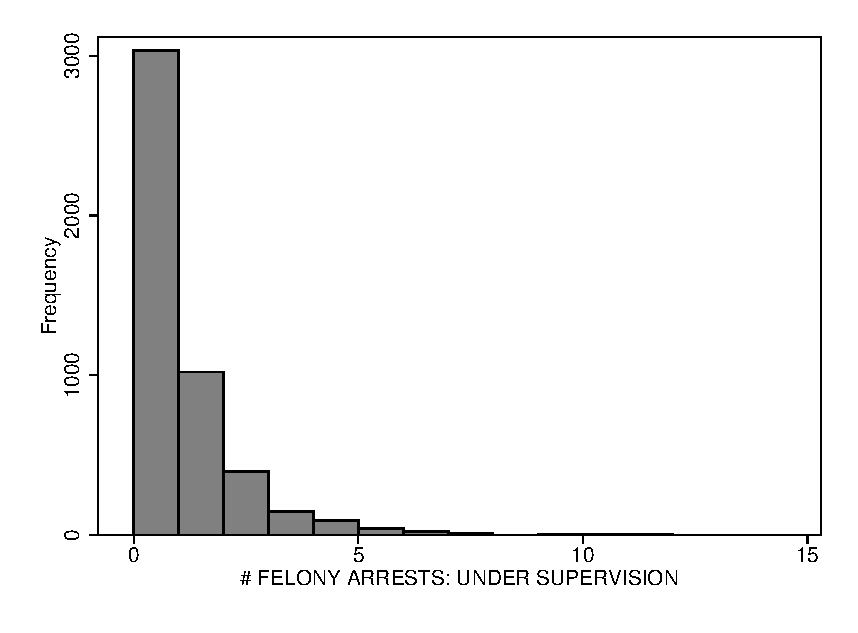
\includegraphics[angle=0,
           width=.75\textwidth]{recdvhist.eps}
   \caption{Distribution of felony recidivism}
  \label{fig:recdvhist}
\end{figure}

\begin{table}[htbp]\centering
\caption{Summary statistics of recidivism data set\label{tab:recddes}
\textbf{} }\begin{tabular} {@{} l cccc @{}} \\
Variable & Mean & SD & Min & Max \\
\hline
Number of arrests &   0.641 &   1.129 &   0.000 &   12.000 \\
Months on probation &   27.880 &   10.932 &   0.067 &   49.500 \\
Risk category (1,2,3) &   1.179 &   0.401 &   1.000 &   3.000 \\
  Female &   0.130 &   0.336 &   0.000 &   1.000 \\
  Never uses drugs & (reference) \\
  Uses drugs occasionally  &   0.220 &   0.414 &   0.000 &   1.000 \\
  Uses drugs frequently &   0.248 &   0.432 &   0.000 &   1.000 \\
   Number of prior felonies &   0.782 &   1.444 &   0.000 &   13.000 \\
  Aged 19 or below & (reference) \\
  Aged 20-24  &   0.305 &   0.460 &   0.000 &   1.000 \\
  Aged 25-29 &   0.228 &   0.419 &   0.000 &   1.000 \\
  Aged 30-39  &   0.225 &   0.418 &   0.000 &   1.000 \\
  Aged 40-49 &   0.077 &   0.266 &   0.000 &   1.000 \\
  Aged 50 plus &   0.043 &   0.203 &   0.000 &   1.000 \\
   Minority &   0.370 &   0.483 &   0.000 &   1.000 \\
    Hispanic &   0.218 &   0.413 &   0.000 &   1.000 \\
\hline
\multicolumn{5}{@{}l}{\footnotesize{\emph{Source:} Recidivism of Felons on Probation 1986-1989}, N = 4,762}
\end{tabular}
\end{table}

\section{Logistic regression}

Our first analysis of the risk of rearrest is to treat the outcome as dichotomous.  Details of the logistic function are given in Chapter~\ref{sec:logit}.  Briefly, the link function estimates the mean outcome as the log-odds
\begin{equation}
\mbox{ln}\left(\frac{p}{1-p}\right)=\beta_0+\sum\beta_px_p
\end{equation}
and once the model is estimated, the exponents of the coefficients are interpreted as a ratio of the odds
\begin{equation}
e^{\beta}=\mbox{odds-ratio}
\end{equation}

Table~\ref{tab:recdlogit} presents the results of the model predicting the chance of rearrest.  According to this model, females are less likely to be rearrested, with an odds ratio ($e^\beta$) of about half the odds.

Compared with those who do not use drugs, the odds of being rearrested increase by about 20 percent for those who use drugs occasionally, and about 80 percent for those who use drugs frequently.

Each prior felony increases the chances of a rearrest, increasing the odds by over 36 percent. Compared to those aged 18 or 19, older individuals are less likely to be rearrested. With each age group, the odds continue to decrease.

The odds of a minority being rearrested are over twice those of someone who is not a minority.  Finally, the odds of someone who is Hispanic are over 50 percent greater than those who are not hispanic.

\begin{table}[htbp]\centering
 \caption{Logistic regression model predicting recidivism \label{tab:recdlogit}}
\begin{tabular}{lcc}
\hline
Variable      &    Model & Odds-Ratio  \\
\hline
Female   &   -0.593***&    0.553***\\
      &   (0.105)  &   (0.058)  \\
Uses drugs occasionally   &    0.212** &    1.237** \\
      &   (0.082)  &   (0.101)  \\
Uses drugs frequently   &    0.602***&    1.825***\\
      &   (0.079)  &   (0.144)  \\
Number of prior felonies    &    0.312***&    1.367***\\
      &   (0.025)  &   (0.034)  \\
Aged 20-24   &   -0.540***&    0.583***\\
      &   (0.103)  &   (0.060)  \\
Aged 25-29   &   -0.729***&    0.482***\\
      &   (0.109)  &   (0.053)  \\
Aged 30-39   &   -1.058***&    0.347***\\
      &   (0.113)  &   (0.039)  \\
Aged 40-49   &   -1.247***&    0.287***\\
      &   (0.158)  &   (0.045)  \\
Aged 50 plus   &   -1.823***&    0.161***\\
      &   (0.229)  &   (0.037)  \\
Minority    &    0.800***&    2.226***\\
      &   (0.074)  &   (0.164)  \\
Hispanic     &    0.446***&    1.562***\\
      &   (0.086)  &   (0.134)  \\
Intercept   &   -0.649***\\
      &   (0.102)  &    \\
\hline
\multicolumn{1}{l}{Model Statistics} \\
\hline
N      &   4762.000  \\
Log-likelihood (null model)    &  -3120.487  \\
Log-likelihood (final model)     &  -2802.139  \\
Pseudo-$R^2$    &    0.102  \\
$\chi^2 LR$    &   636.697  \\
$df$ Regression    &    11.000  \\
\hline
\multicolumn{3}{l}{$SE$s in parentheses, $**p<0.01, ***p<0.001$} \\
\hline
\end{tabular}
\end{table}

\section{Probit regression}

Another method

\begin{table}[htbp]\centering
 \caption{Probit regression model predicting recidivism \label{tab:recdprob}}
\begin{tabular}{lc}
\hline
Variable      &    Model  \\
\hline
Female   &   -0.348***\\
      &   (0.061)  \\
Uses drugs occasionally   &    0.133** \\
      &   (0.049)  \\
Uses drugs frequently   &    0.369***\\
      &   (0.048)  \\
Number of prior felonies    &    0.183***\\
      &   (0.014)  \\
Aged 20-24   &   -0.330***\\
      &   (0.063)  \\
Aged 25-29   &   -0.446***\\
      &   (0.067)  \\
Aged 30-39   &   -0.641***\\
      &   (0.069)  \\
Aged 40-49   &   -0.747***\\
      &   (0.093)  \\
Aged 50 plus   &   -1.082***\\
      &   (0.128)  \\
Minority    &    0.483***\\
      &   (0.044)  \\
Hispanic     &    0.270***\\
      &   (0.051)  \\
Intercept    &   -0.395***\\
      &   (0.063)  \\
\hline
\multicolumn{1}{l}{Model Statistics} \\
\hline
N      &   4762.000  \\
Log-likelihood (null model)    &  -3120.487  \\
Log-likelihood (final model)     &  -2802.980  \\
Pseudo-$R^2$    &    0.102  \\
$\chi^2 LR$    &   635.014  \\
$df$ Regression    &    11.000  \\
\hline
\multicolumn{2}{l}{$SE$s in parentheses, $**p<0.01, ***p<0.001$} \\
\hline
\end{tabular}
\end{table}

\section{Poisson regression}

\begin{table}[htbp]\centering
 \caption{Poisson regression model predicting recidivism \label{tab:recdpois}}
 \begin{tabular}{lcccc}
\hline
Variable      &    Model1 & Rate-Ratio &    Model2 & Rate-Ratio  \\
\hline
Female   &   -0.391***&    0.676***&   -0.432***&    0.649***\\
      &   (0.065)  &   (0.044)  &   (0.065)  &   (0.042)  \\
Uses drugs occasionally   &    0.133** &    1.142** &    0.159***&    1.172***\\
      &   (0.048)  &   (0.055)  &   (0.048)  &   (0.056)  \\
Uses drugs frequently   &    0.514***&    1.673***&    0.574***&    1.775***\\
      &   (0.042)  &   (0.071)  &   (0.042)  &   (0.075)  \\
Number of prior felonies    &    0.129***&    1.138***&    0.141***&    1.152***\\
      &   (0.009)  &   (0.010)  &   (0.009)  &   (0.010)  \\
Aged 20-24   &   -0.314***&    0.730***&   -0.335***&    0.716***\\
      &   (0.053)  &   (0.039)  &   (0.053)  &   (0.038)  \\
Aged 25-29   &   -0.422***&    0.656***&   -0.477***&    0.621***\\
      &   (0.057)  &   (0.038)  &   (0.057)  &   (0.035)  \\
Aged 30-39   &   -0.605***&    0.546***&   -0.636***&    0.529***\\
      &   (0.061)  &   (0.033)  &   (0.060)  &   (0.032)  \\
Aged 40-49   &   -0.934***&    0.393***&   -1.064***&    0.345***\\
      &   (0.101)  &   (0.040)  &   (0.101)  &   (0.035)  \\
Aged 50 plus   &   -1.503***&    0.223***&   -1.629***&    0.196***\\
      &   (0.170)  &   (0.038)  &   (0.170)  &   (0.033)  \\
Minority    &    0.577***&    1.781***&    0.657***&    1.928***\\
      &   (0.042)  &   (0.076)  &   (0.042)  &   (0.082)  \\
Hispanic     &    0.370***&    1.448***&    0.448***&    1.565***\\
      &   (0.050)  &   (0.072)  &   (0.050)  &   (0.078)  \\
Intercept    &   -0.634***&   &   -3.987***&    \\
      &   (0.056)  &   &   (0.057)  &    \\
\hline
\multicolumn{4}{l}{Model Statistics} \\
\hline
N      &  4762.000  &   &  4762.000  &   \\
Log-likelihood (null model)    &  -5707.894  &   &  -6121.835   \\
Log-likelihood (final model)     &  -5253.794  &   &  -5550.715  \\
Pseudo-$R^2$    &    0.080  &    &    0.093  &     \\
$\chi^2 LR$    &   908.200  &   &  1142.240  &   \\
$df$ Regression    &   11.000  &    &   11.000  &    \\
\hline
\multicolumn{4}{l}{Model 2 includes time exposure variable} \\
\multicolumn{4}{l}{$SE$s in parentheses, $**p<0.01, ***p<0.001$} \\
\hline
\end{tabular}
\end{table}

\section{Negative binomial regression}

\begin{table}[htbp]\centering
 \caption{Negative binomial regression model predicting recidivism \label{tab:recdnb}}
 \begin{tabular}{lcccc}
\hline
Variable      &    Model1 & Rate-Ratio &    Model2 & Rate-Ratio  \\
\hline
Female   &   -0.392***&    0.675***&   -0.418***&    0.659***\\
      &   (0.081)  &   (0.055)  &   (0.087)  &   (0.057)  \\
Uses drugs occasionally   &    0.163** &    1.177** &    0.219** &    1.245** \\
      &   (0.062)  &   (0.073)  &   (0.068)  &   (0.084)  \\
Uses drugs frequently   &    0.545***&    1.725***&    0.656***&    1.927***\\
      &   (0.057)  &   (0.099)  &   (0.062)  &   (0.120)  \\
Number of prior felonies    &    0.164***&    1.178***&    0.190***&    1.209***\\
      &   (0.015)  &   (0.018)  &   (0.017)  &   (0.021)  \\
Aged 20-24   &   -0.334***&    0.716***&   -0.432***&    0.650***\\
      &   (0.074)  &   (0.053)  &   (0.082)  &   (0.053)  \\
Aged 25-29   &   -0.447***&    0.639***&   -0.602***&    0.547***\\
      &   (0.079)  &   (0.051)  &   (0.087)  &   (0.047)  \\
Aged 30-39   &   -0.661***&    0.516***&   -0.814***&    0.443***\\
      &   (0.083)  &   (0.043)  &   (0.091)  &   (0.040)  \\
Aged 40-49   &   -0.979***&    0.376***&   -1.203***&    0.300***\\
      &   (0.124)  &   (0.047)  &   (0.133)  &   (0.040)  \\
Aged 50 plus   &   -1.603***&    0.201***&   -1.907***&    0.148***\\
      &   (0.194)  &   (0.039)  &   (0.205)  &   (0.030)  \\
Minority    &    0.587***&    1.799***&    0.712***&    2.038***\\
      &   (0.055)  &   (0.099)  &   (0.060)  &   (0.122)  \\
Hispanic     &    0.380***&    1.462***&    0.484***&    1.623***\\
      &   (0.065)  &   (0.094)  &   (0.070)  &   (0.114)  \\
Intercept    &   -0.663***&    0.515***&   -3.909***&    0.020***\\
      &   (0.075)  &   (0.039)  &   (0.082)  &   (0.002)  \\
$\alpha$  &    1.007 & &      1.291*** \\
       &   (0.066)  & &   (0.077)  \\
\hline
\multicolumn{4}{l}{Model Statistics} \\
\hline
N      &  4762.000  &   &  4762.000  &   \\
Log-likelihood (null model)    &  -5204.197  &   & -5434.993   \\
Log-likelihood (final model)     & -4935.635  &   &  -5119.788    \\
Pseudo-$R^2$    &    0.052  &    &    0.058  &     \\
$\chi^2 LR$    &   537.124  &   &  630.411  &   \\
$df$ Regression    &   11.000  &    &   11.000  &    \\
\hline
\multicolumn{4}{l}{Model 2 includes time exposure variable} \\
\multicolumn{4}{l}{$SE$s in parentheses, $**p<0.01, ***p<0.001$} \\
\hline
\end{tabular}
\end{table}

\section{Zero-inflated Poisson regression}

\begin{table}[htbp]\centering
 \caption{Poisson model predicting level of recidivism in ZIP regression \label{tab:recdzip}}
\begin{tabular}{lcc}
\hline
Variable      &    Model & Rate-Ratio  \\
\hline
Female   &   -0.057  &    0.944  \\
      &   (0.087)  &   (0.082)  \\
Uses drugs occasionally   &   -0.034  &    0.966  \\
      &   (0.064)  &   (0.061)  \\
Uses drugs frequently   &    0.311***&    1.365***\\
      &   (0.054)  &   (0.073)  \\
Number of prior felonies    &    0.017  &    1.017  \\
      &   (0.011)  &   (0.012)  \\
Aged 20-24   &   -0.170* &    0.843* \\
      &   (0.067)  &   (0.056)  \\
Aged 25-29   &   -0.243***&    0.784***\\
      &   (0.073)  &   (0.057)  \\
Aged 30-39   &   -0.152* &    0.859* \\
      &   (0.077)  &   (0.066)  \\
Aged 40-49   &   -0.603***&    0.547***\\
      &   (0.147)  &   (0.080)  \\
Aged 50 plus   &   -0.849***&    0.428***\\
      &   (0.246)  &   (0.105)  \\
Minority    &    0.323***&    1.382***\\
      &   (0.055)  &   (0.076)  \\
Hispanic     &    0.257***&    1.293***\\
      &   (0.065)  &   (0.084)  \\
Intercept    &   -3.181***&    0.042***\\
      &   (0.073)  &   (0.003)  \\
\hline
\multicolumn{1}{l}{Model Statistics} \\
\hline
N      &   4762.000  \\
Log-likelihood (null model)    &  -5224.913  \\
Log-likelihood (final model)     &  -5164.957  \\
$\chi^2 LR$    &   119.913  \\
$df$ Regression    &    11.000  \\
\hline
\multicolumn{3}{l}{Inflation portion of model presented in Table~\ref{tab:recdinflate}} \\
\multicolumn{3}{l}{$SE$s in parentheses, $*p<0.05, ***p<0.001$} \\
\hline
\end{tabular}
\end{table}

\begin{table}[htbp]\centering
 \caption{Logistic model predicting no recidivism in ZIP regression \label{tab:recdinflate}}
\begin{tabular}{lcc}
\hline
Variable      &    Model & Odds-Ratio  \\
\hline
Female   &    0.697***&    2.008***\\
      &   (0.152)  &   (0.306)  \\
Uses drugs occasionally   &   -0.438** &    0.645** \\
      &   (0.139)  &   (0.090)  \\
Uses drugs frequently   &   -0.607***&    0.545***\\
      &   (0.123)  &   (0.067)  \\
Number of prior felonies    &   -0.754***&    0.471***\\
      &   (0.077)  &   (0.036)  \\
Aged 20-24   &    0.611***&    1.842***\\
      &   (0.167)  &   (0.308)  \\
Aged 25-29   &    0.827***&    2.286***\\
      &   (0.177)  &   (0.404)  \\
Aged 30-39   &    1.338***&    3.810***\\
      &   (0.176)  &   (0.672)  \\
Aged 40-49   &    1.147***&    3.149***\\
      &   (0.270)  &   (0.849)  \\
Aged 50 plus   &    1.714***&    5.551***\\
      &   (0.378)  &   (2.100)  \\
Minority    &   -0.809***&    0.445***\\
      &   (0.117)  &   (0.052)  \\
Hispanic     &   -0.437** &    0.646** \\
      &   (0.134)  &   (0.087)  \\
Intercept    &    0.091  &    1.095  \\
      &   (0.166)  &   (0.182)  \\
\hline
\multicolumn{3}{l}{$SE$s in parentheses, $**p<0.01, ***p<0.001$} \\
\hline
\end{tabular}
\end{table}

\section{Ordered logistic regression}


\begin{table}[htbp]\centering
 \caption{Ordered logistic regression model predicting risk level \label{tab:recdologit}}
\begin{tabular}{lcc}
\hline
Variable      &    Model & Odds-Ratio  \\
\hline
Female   &   -0.069  &    0.934  \\
      &   (0.142)  &   (0.132)  \\
Uses drugs occasionally   &    1.306***&    3.690***\\
      &   (0.121)  &   (0.445)  \\
Uses drugs frequently   &    2.292***&    9.890***\\
      &   (0.114)  &   (1.130)  \\
Number of prior felonies    &    0.250***&    1.283***\\
      &   (0.026)  &   (0.033)  \\
Aged 20-24   &   -1.965***&    0.140***\\
      &   (0.123)  &   (0.017)  \\
Aged 25-29   &   -2.851***&    0.058***\\
      &   (0.148)  &   (0.009)  \\
Aged 30-39   &   -2.882***&    0.056***\\
      &   (0.152)  &   (0.009)  \\
Aged 40-49   &   -2.641***&    0.071***\\
      &   (0.229)  &   (0.016)  \\
Aged 50 plus   &   -2.328***&    0.097***\\
      &   (0.298)  &   (0.029)  \\
Minority    &    0.317** &    1.373** \\
      &   (0.098)  &   (0.134)  \\
Hispanic     &   -0.269* &    0.764* \\
      &   (0.122)  &   (0.094)  \\ \hline
cut 1    &        &        \\
Intercept    &    1.016***&    \\
      &   (0.121)  &   \\
cut 2    &        &        \\
Intercept    &    4.984***&   \\
      &   (0.212)  &   \\
\hline
\multicolumn{1}{l}{Model Statistics} \\
\hline
N      &   4762.000  \\
Log-likelihood (null model)    &  -2324.205  \\
Log-likelihood (final model)     &  -1782.966   \\
Pseudo-$R^2$    &    0.233  \\
$\chi^2 LR$    &   1082.479  \\
$df$ Regression    &    11.000  \\
\hline
\multicolumn{3}{l}{$SE$s in parentheses, $*p<0.05, **p<0.01, ***p<0.001$} \\
\hline
\end{tabular}
\end{table}

\section{Multinomial logistic regression}

\begin{table}[htbp]\centering
 \caption{Multinomial logistic regression model predicting risk level \label{tab:recdmul}}
 \begin{tabular}{lcccc}
\hline
Variable      &    Med. & Rel.-Risk-Ratio &    High & Rel.-Risk-Ratio  \\
\hline
Female   &   -0.065  &    0.937  &   -0.115  &    0.891  \\
      &   (0.144)  &   (0.135)  &   (0.632)  &   (0.564)  \\
Uses drugs occasionally   &    1.301***&    3.673***&    1.646* &    5.188* \\
      &   (0.122)  &   (0.449)  &   (0.656)  &   (3.405)  \\
Uses drugs frequently   &    2.255***&    9.534***&    3.651***&   38.523***\\
      &   (0.117)  &   (1.112)  &   (0.568)  &  (21.866)  \\
Number of prior felonies    &    0.266***&    1.305***&    0.114  &    1.120  \\
      &   (0.027)  &   (0.035)  &   (0.151)  &   (0.170)  \\
Aged 20-24   &   -2.012***&    0.134***&   -2.174***&    0.114***\\
      &   (0.127)  &   (0.017)  &   (0.388)  &   (0.044)  \\
Aged 25-29   &   -2.814***&    0.060***&   -18.762  &    0.000  \\
      &   (0.152)  &   (0.009)  &  (981.878)  &   (0.000)  \\
Aged 30-39   &   -2.840***&    0.058***&   -18.824  &    0.000  \\
      &   (0.156)  &   (0.009)  &  (989.152)  &   (0.000)  \\
Aged 40-49   &   -2.600***&    0.074***&   -18.269  &    0.000  \\
      &   (0.231)  &   (0.017)  & (1762.055)  &   (0.000)  \\
Aged 50 plus   &   -2.282***&    0.102***&   -17.933  &    0.000  \\
      &   (0.300)  &   (0.031)  & (2429.416)  &   (0.000)  \\
Minority    &    0.313** &    1.367** &    0.451  &    1.570  \\
      &   (0.100)  &   (0.136)  &   (0.394)  &   (0.619)  \\
Hispanic     &   -0.244* &    0.783* &   -0.782  &    0.457  \\
      &   (0.124)  &   (0.097)  &   (0.586)  &   (0.268)  \\
Intercept    &   -1.051***&    &   -4.465***&    \\
      &   (0.123)  &    &   (0.585)  &   \\
\hline
\multicolumn{4}{l}{Model Statistics} \\
\hline
N      &  4762.000   \\
Log-likelihood (null model)    &  -2324.205   \\
Log-likelihood (final model)     & -1766.584   \\
Pseudo-$R^2$    &    0.240 \\
$\chi^2 LR$    &   1115.242  &     \\
$df$ Regression    &   22.000  &      \\
\hline
\multicolumn{4}{l}{Reference outcome is low risk} \\
\multicolumn{4}{l}{$SE$s in parentheses, $*p<0.05, **p<0.01, ***p<0.001$} \\
\hline
\end{tabular}
\end{table}


\section{A note on interactions}